\chapter{Desarrollo}

El desarrollo del Ejercicio Práctico N° 4 consiste en el diseño e implementación de un sistema de comunicación
serie bidireccional asíncrono entre la placa de desarrollo BluePill (STM32F103) y una PC.

\section{Descripción General del Funcionamiento}

El sistema funciona de manera interactiva a través del puerto serie configurado a $9600$ baudios con formato de
trama 8N1. Al iniciar la ejecución o al presionar el botón de reset de la BluePill, el microcontrolador envía un
mensaje de bienvenida a la PC detallando el menú de opciones disponibles.

La interacción se controla mediante una máquina de estados implementada en el bucle principal de la BluePill:
\begin{itemize}
  \item \textbf{Estado S0 (MENÚ):} El microcontrolador espera recibir un comando desde la terminal. Si recibe la
        letra `A' o `a', transiciona al estado S1. Si recibe la letra `B' o `b', transiciona al estado S2.
  \item \textbf{Estado S1 (TOGGLE BLINK):} Habilita o deshabilita el parpadeo del LED integrado en la placa
        (conectado al pin GPIOC13). El parpadeo se realiza mediante una comparación temporal utilizando la variable
        \lstinline{ticks} del controlador de SysTick (intervalos de \qty{500}{\ms}). Seguidamente, transiciona al estado S3.
  \item \textbf{Estado S2 (ECHO):} El microcontrolador reenvía inmediatamente cualquier cadena recibida,
        anteponiendo la cabecera \texttt{"ECHO: "}. Este modo se mantiene activo de forma interactiva hasta que el
        usuario envía la palabra reservada \texttt{"SALIR"}, momento en el cual transiciona al estado S3.
  \item \textbf{Estado S3 (RETURN):} Imprime nuevamente las opciones del menú de selección en la pantalla de la PC y
        retorna al estado S0 para esperar la siguiente entrada del usuario.
\end{itemize}

El procesamiento de las cadenas recibidas por la UART utiliza un búfer circular (anillo) estático de
\qty{256}{\byte}. Los bytes entrantes se guardan de forma asíncrona dentro de la ISR de recepción (`RXNE'). El
bucle de control principal en `main' consulta periódicamente la presencia del carácter de terminación `\textbackslash n'
en el búfer circular sin bloquear el procesador ni realizar asignación dinámica de memoria (\textit{malloc}), evitando
la fragmentación de la SRAM del microcontrolador.

\section{Esquema de Conexión Físico}

Para establecer la comunicación entre la placa BluePill y la PC, es necesario emplear un circuito conversor físico
USB-UART CP2102. Los niveles lógicos de la BluePill operan a voltajes de \qty{3.3}{\V}, compatibles con este conversor.

La conexión requiere realizar un cruzamiento de las líneas de transmisión y recepción de datos, además de unir las
referencias de tierra para garantizar la integridad de las señales eléctricas. La figura~\ref{fig:conexion_uart}
representa el conexionado físico realizado:
\begin{itemize}
  \item Pin \textbf{PA9} (USART1\_TX) de la BluePill al pin \textbf{RXD} (entrada) del conversor.
  \item Pin \textbf{PA10} (USART1\_RX) de la BluePill al pin \textbf{TXD} (salida) del conversor.
  \item Pin \textbf{GND} de la BluePill al pin \textbf{GND} del conversor.
\end{itemize}

\begin{figure}[!ht]
  \centering
  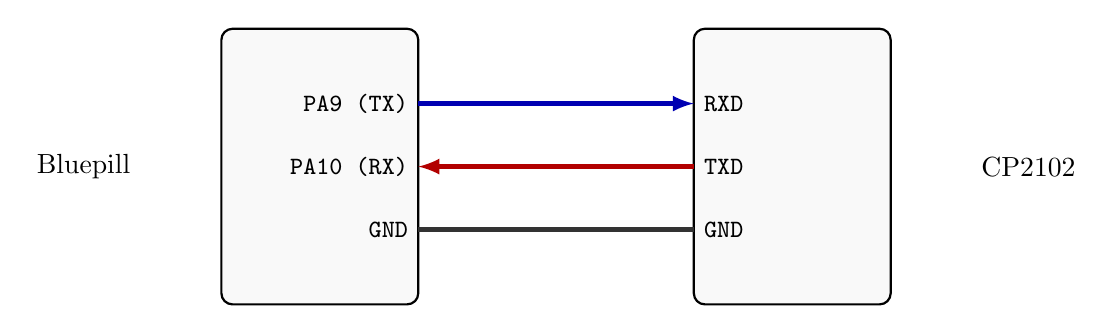
\begin{tikzpicture}[
    >=latex, 
    thick,
    box/.style={draw, rectangle, minimum height=3.5cm, minimum width=2.5cm, align=center, fill=gray!5, rounded corners},
    pinlabel/.style={font=\ttfamily\small}
]
  
  % Nodo BluePill
  \node[box] (bp) at (0,0) {};
  \node[] (lab1a) at (-3,0) {Bluepill};
  
  % Pines en la BluePill
  \node[anchor=east, pinlabel] at (1.25, 0.8)  (bp_tx)  {PA9 (TX) };
  \node[anchor=east, pinlabel] at (1.25, 0.0)  (bp_rx)  {PA10 (RX)};
  \node[anchor=east, pinlabel] at (1.25, -0.8) (bp_gnd) {GND      };
  
  % Nodo Conversor USB-UART
  \node[box] (conv) at (6,0) {};
  \node[] (lab1b) at (9,0) {CP2102};
  
  % Pines en el Conversor
  \node[anchor=west, pinlabel] at (4.75, 0.8)  (conv_rx)  { RXD};
  \node[anchor=west, pinlabel] at (4.75, 0.0)  (conv_tx)  { TXD};
  \node[anchor=west, pinlabel] at (4.75, -0.8) (conv_gnd) { GND};
  
  % Conexiones con flechas y colores
  \draw[->, color=blue!70!black, ultra thick] (1.25, 0.8) -- (4.75, 0.8);
  \draw[<-, color=red!70!black, ultra thick] (1.25, 0.0) -- (4.75, 0.0);
  \draw[-, color=black!80, ultra thick] (1.25, -0.8) -- (4.75, -0.8);
  
\end{tikzpicture}

  \caption{Esquema de conexión física entre el microcontrolador STM32F103 y el conversor USB-UART CP2102.}
  \label{fig:conexion_uart}
\end{figure}

\section{Configuración del Periférico USART1}

La configuración del periférico USART1 en el STM32F103 se realiza manipulando directamente los registros de control
provistos por el estándar CMSIS.

\subsection{Habilitación de Clocks y Configuración de Pines GPIO}
El USART1 se encuentra conectado al bus periférico de alta velocidad APB2. Por lo tanto, el primer paso consiste en
habilitar el clock del periférico y del puerto GPIOA en el registro de control de reloj:
\begin{lstlisting}[language=C]
RCC->APB2ENR |= RCC_APB2ENR_USART1EN | RCC_APB2ENR_IOPAEN;
\end{lstlisting}

Los pines asociados a la función alternativa de la USART1 en el puerto A son PA9 (TX) y PA10 (RX). De acuerdo a las
especificaciones de hardware del manual de referencia (RM0008) de STMicroelectronics:
\begin{itemize}
  \item \textbf{PA9 (TX):} Debe configurarse como salida digital con función alternativa push-pull y una velocidad
        máxima de \qty{50}{\MHz} (bits de configuración \lstinline{CNF9 = 0b10} y \lstinline{MODE9 = 0b11}, equivalente a la máscara hexadecimal \lstinline{0xB}).
  \item \textbf{PA10 (RX):} Debe configurarse como entrada digital flotante o con resistencia de pull-up interna
        (se optó por entrada con pull-up para evitar ruidos cuando el cable está desconectado, configurando
        \lstinline{CNF10 = 0b10} y \lstinline{MODE10 = 0b00}, equivalente a \lstinline{0x4}, habilitando el bit \lstinline{ODR10} en $1$).
\end{itemize}
Esta configuración se realiza en el registro de control alto del puerto A (\lstinline{GPIOA->CRH}).

\subsection{Cálculo del Baudrate (Registro USART\_BRR)}
La tasa de transmisión del puerto serie se configura mediante el registro divisor de baudios \lstinline{USART1->BRR}.
Dado que el microcontrolador arranca en su estado por defecto utilizando el oscilador interno (HSI) a una frecuencia de
reloj del sistema de $f_{\text{CK}} = 8\MHz$, y la USART1 está conectada directamente al bus APB2 (cuyo prescaler es
1 por defecto), la frecuencia de reloj del periférico es $8\MHz$.

La fórmula general para el cálculo de la tasa de baudios en la arquitectura STM32 es:
\begin{equation}
  \text{Baud Rate} = \frac{f_{\text{CK}}}{16 \times \text{USARTDIV}}
\end{equation}

Despejando el factor divisor de reloj $\text{USARTDIV}$ para una velocidad deseada de $9600$ baudios:
\begin{equation}
  \text{USARTDIV} = \frac{8,000,000}{16 \times 9600} \approx 52.0833
\end{equation}

El registro \lstinline{USART_BRR} divide su contenido de 16 bits en dos partes:
\begin{itemize}
  \item \textbf{Mantisa (bits [15:4]):} La parte entera de $\text{USARTDIV}$. En este caso, $52 = \text{0x34}$.
  \item \textbf{Fracción (bits [3:0]):} La parte decimal multiplicada por 16 y redondeada al entero más cercano.
        \begin{equation}
          \text{Fracción} = 0.0833 \times 16 = 1.332 \approx 1 = \text{0x1}
        \end{equation}
\end{itemize}
Combinando ambos campos, el valor a escribir en el registro es \lstinline{USART1->BRR = 0x341;}.

\subsection{Formato de Trama y Habilitación}
El formato de trama 8N1 (8 bits de datos, sin paridad, 1 bit de parada) se parametriza en los registros de control:
\begin{itemize}
  \item \textbf{8 bits de datos:} Se limpia el bit \lstinline{M} (Word length) en \lstinline{USART1->CR1}.
  \item \textbf{Sin paridad:} Se limpia el bit \lstinline{PCE} (Parity control enable) en \lstinline{USART1->CR1}.
  \item \textbf{1 bit de parada:} Se limpian los bits de parada \lstinline{STOP[1:0]} en \lstinline{USART1->CR2}.
\end{itemize}

Finalmente, se activan los bloques internos de transmisión (\lstinline{TE}) y recepción (\lstinline{RE}), se
habilitan las interrupciones por hardware para recepción de dato disponible (\lstinline{RXNEIE}) y transmisión
completa (\lstinline{TCIE}), y se energiza el periférico activando el bit de habilitación general (\lstinline{UE}):
\begin{lstlisting}[language=C]
USART1->CR1 = USART_CR1_TCIE | USART_CR1_RXNEIE | USART_CR1_RE | USART_CR1_TE;
USART1->CR1 |= USART_CR1_UE;
NVIC_EnableIRQ(USART1_IRQn);
\end{lstlisting}

\section{Aplicación del Lado de la PC}

Para interactuar con la placa de desarrollo desde la PC, se desarrolló una aplicación simplificada en C
para sistemas operativos basados en Linux. La aplicación abre de forma directa el puerto serie configurado en
la ruta física \texttt{/dev/ttyUSB0} mediante la llamada al sistema \lstinline{open()}.

La configuración del puerto serie se realiza a través de las estructuras y llamadas provistas por la biblioteca
\texttt{<termios.h>}. El puerto se parametriza a una velocidad de $9600$ baudios (tanto de entrada como de salida)
y en formato de trama 8N1 (8 bits de datos, sin paridad, 1 bit de parada), deshabilitando el control de flujo
por hardware o software y forzando el modo de operación crudo (\textit{raw mode}) mediante \lstinline{cfmakeraw()}.

Para lograr una comunicación bidireccional interactiva en tiempo real (full-duplex) en un único proceso y de forma
eficiente, se utiliza la llamada al sistema \lstinline{poll()} de Linux. Se configuran dos descriptores de archivo
a monitorear:
\begin{enumerate}
  \item \textbf{Entrada Estándar (\texttt{STDIN\_FILENO}):} Monitorea cuando el usuario escribe en la consola. Al
        presionar Enter, el carácter introducido (incluyendo el retorno \lstinline{'\n'} por estar la terminal de la PC en
        modo canónico) se lee desde el teclado y se escribe directamente en el puerto serie hacia la BluePill.
  \item \textbf{Descriptor del Puerto Serie (\texttt{fd}):} Monitorea la recepción asíncrona de datos desde el
        microcontrolador. Al llegar un byte, se lee del puerto y se vuelca de inmediato en la salida estándar de
        la terminal mediante \lstinline{putchar()} y \lstinline{fflush(stdout)}.
\end{enumerate}

El código fuente de la aplicación para la PC se encuentra en el listado~\ref{list.ej4:pc_monitor}.

\section{Pruebas Realizadas}

Para validar el comportamiento del sistema completo se llevaron a cabo los siguientes ensayos utilizando la
aplicación terminal interactiva en la PC conectada a la BluePill:
\begin{itemize}
  \item \textbf{Prueba de arranque y transmisión:} Al alimentar o resetear la placa, se verificó la recepción del
        mensaje de bienvenida:
        \begin{verbatim}
        Terminal Bluepill
        Seleccione una de las opciones:
         A. Parpadeo GPIOC13
         B. Echo
        Opcion:
        \end{verbatim}
  \item \textbf{Prueba del Comando A (Blink):} Se ingresó la opción `A' en la terminal de la PC. El sistema procesó la
        entrada, alternó el flag de parpadeo, y respondió enviando el texto \texttt{"-- Blink ON --"} (o \texttt{"-- Blink OFF --"}),
        mostrando de nuevo el menú. Físicamente, se constató que el LED verde de la placa (pin PC13) comenzó a parpadear a una frecuencia de
        \qty{1}{\Hz} ($500\ms$ encendido y $500\ms$ apagado) de forma precisa y estable.
  \item \textbf{Prueba del Comando B (Modo Echo):} Se ingresó la opción `B'. El microcontrolador respondió con
        el mensaje informativo. A partir de allí, cualquier texto enviado (por ejemplo: \texttt{"Hola Mundo"}) fue devuelto
        por la placa e impreso en la terminal de la PC como \texttt{"ECHO: Hola Mundo"}.
  \item \textbf{Prueba de salida del modo Echo:} Dentro del modo eco, se ingresó el comando \texttt{"SALIR"}. La placa
        procesó la comparación de cadenas de forma exitosa, envió el texto \texttt{"Saliendo..."} y retornó al menú principal.
  \item \textbf{Prueba de robustez y límites de búfer:} Se enviaron mensajes con longitudes superiores a los
        \qty{16}{\byte} permitidos por el búfer de lectura en el main. Se verificó que el sistema copió únicamente los primeros
        16 caracteres útiles, descartó de forma segura el resto de los bytes sobrantes hasta encontrar el terminador `\textbackslash n',
        y continuó operando de manera normal sin sufrir desbordamiento del anillo ni bloqueos del microcontrolador.
\end{itemize}

\section{Código Fuente del Proyecto}

A continuación, se adjuntan los códigos fuente completos implementados para ambos lados de la comunicación:

\lstinputlisting[language={C}, caption={Código fuente del microcontrolador STM32F103 en BareMetal/CMSIS (\texttt{main.c}).}, label={list.ej4:main}]{sources/src/main.c}

\lstinputlisting[language={C}, caption={Código fuente del monitor de terminal en la PC (\texttt{serial\_monitor.c}).}, label={list.ej4:pc_monitor}]{sources/src/serial_monitor.c}
